%%%%%%%%%%%%%%%%%%%%%%%%%%%%%%%%%%%%%%%%%%%%%%%%%%%%%%%%%%%%%%%%%%%%%%%%%%%%%%%%%%%%%%%%%%%%%%%%%%%%%%%%%%%%%%%%%%%%%%%%%%%%%%%%%%%%%%%%%%%%%%%%%%%%%%
% 20141001 - Introduction to Operating Systems VO
%%%%%%%%%%%%%%%%%%%%%%%%%%%%%%%%%%%%%%%%%%%%%%%%%%%%%%%%%%%%%%%%%%%%%%%%%%%%%%%%%%%%%%%%%%%%%%%%%%%%%%%%%%%%%%%%%%%%%%%%%%%%%%%%%%%%%%%%%%%%%%%%%%%%%%

%fancyhdr
\lhead{IOS VO} 
\rhead{2014-10-01}

%%%%%%%%%%%%%%%%%%%%%%%%%%%%%%%%%%%%%%%%%%%%%%%%%%%%%%%%%%%%%%%%%%%%%%%%%%%%%%%%%%%%%%%%%%%%%%%%%%%%%%%%%%%%%%%%%%%%%%%%%%%%%%%%%%%%%%%%%%%%%%%%%%%%%%

\section*{Myth Busting}

%%%%%%%%%%%%%%%%%%%%%%%%%%%%%%%%%%%%%%%%%%%%%%%%%%%%%%%%%%%%%%%%%%%%%%%%%%%%%%%%%%%%%%%%%%%%%%%%%%%%%%%%%%%%%%%%%%%%%%%%%%%%%%%%%%%%%%%%%%%%%%%%%%%%%%

\begin{mb}
	\myth{I prefer programming language X because it makes it more convenient to implement my application.}
	\answer{Wrong!}
\end{mb}

\par{
	\noindent
	The fundamental problem of programming is to establish functional \underline{correctness} and adequate \underline{performance}. Different languages provide different tools of automating the process of establishing correctness and performance. The language should be chosen based on that insight.
}

\par{
	\begin{figure}[!htb]
		\centering
		\begin{tikzpicture}[scale = 1.0]
			\draw (0, 2) rectangle (2, 4) node[pos = 0.5]{\textit{Tool}};

			\node (code) at (1, 0) {\textit{Code}};
			\draw[->] (1, 2) -- (1, 0.25);

			\node (program) at (1, 6) {\textit{Program}};
			\draw[->] (1, 5.75) -- (1, 4);

			\draw (2.1, 3) -- (9, 3);
			\node (compiletime) at (10, 4) {\textit{Compile time}};
			\node (runtime) at (10, 2) {\textit{Runtime}};
			\node (correctnessgenerated) at (5, 4.5) [text width = 3cm]{\textit{Check correctness and generate code}};
			\node (executecorrectness) at (5, 1.5) [text width = 3cm]{\textit{Executes and checks correctness}};
		\end{tikzpicture}
		\caption{Process of establishing correctness.}
		\label{fig:processcorrectness}
	\end{figure}
}

\par{
	\noindent
	\underline{Ultimate goal:} \newline
	A Compiler checking correctness in such a sense that no exception is thrown while executing in any case. But this is infeasible (mathematical proof possible).
}

\par{
	\noindent
	Hardware Exception: Interrupts, a mechanism to stop memory accesses in hardware.
}

%%%%%%%%%%%%%%%%%%%%%%%%%%%%%%%%%%%%%%%%%%%%%%%%%%%%%%%%%%%%%%%%%%%%%%%%%%%%%%%%%%%%%%%%%%%%%%%%%%%%%%%%%%%%%%%%%%%%%%%%%%%%%%%%%%%%%%%%%%%%%%%%%%%%%%

\begin{mb}
	\myth{I like garbage-collected languages like Java because they free me from memory management.}
	\answer{Wrong!}
\end{mb}

\par{
	\noindent
	A garbage collector (GC) provides safe deallocation of unneeded memory but the programmer still needs to say what is unneeded, otherwise the system will run out of memory (memory leak).
}

\par{
	\begin{figure}[!htb]
		\centering
		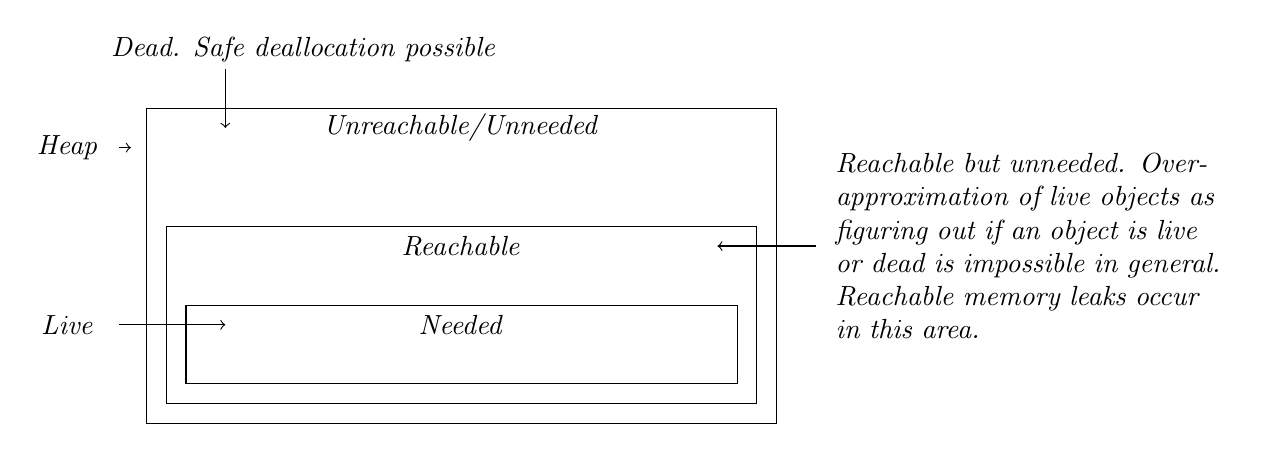
\begin{tikzpicture}[scale = 1.0]
			\draw (1, 4) rectangle (9, 8);
			\node (unreachable) at (5, 7.75) {\textit{Unreachable/Unneeded}};

			\draw (1.25, 4.25) rectangle (8.75, 6.5);
			\node (reachable) at (5, 6.25) {\textit{Reachable}};

			\draw (1.5, 4.5) rectangle (8.5, 5.5);
			\node (needed) at (5, 5.25) {\textit{Needed}};

			\draw[->] (0.65, 7.5) -- (0.8, 7.5);
			\node (heap) at (0, 7.5) {\textit{Heap}};

			\draw[->] (0.65, 5.25) -- (2, 5.25);
			\node (live) at (0, 5.25) {\textit{Live}};

			\draw[->] (2, 8.5) -- (2, 7.75);
			\node (dead) at (3, 8.75) {\textit{Dead. Safe deallocation possible}};

			\draw[->] (9.5, 6.25) -- (8.25, 6.25);
			\node (reachableunneeded) at (12.25, 6.25) [text width = 5cm]{\textit{Reachable but unneeded. Overapproximation of live objects as figuring out if an object is live or dead is impossible in general. Reachable memory leaks occur in this area.}};
		\end{tikzpicture}
		\caption{Unreachable, reachable and needed set of a program.}
		\label{fig:reachablesetprogram}
	\end{figure}
}

\par{
	\noindent
	General runtime complexity of a garbage collector: the size of the heap.
}

\subsection*{Multicore}

\par{
	\noindent
	Amdahl's Law: $P$ represents program parallelism on $N$ cores
	\parskip0pt\begin{itemize}
		\item{$S(N) = N$ if $P = 100\%$. This is ideal multicore scalability.}
		\item{In general: $S(N) = \frac{1}{(1 - P) \cdot \frac{P}{N}}$}
	\end{itemize}
}

\par{
	\begin{figure}[!htb]
		\centering
		\begin{tikzpicture}[scale = 1.75]
			% axes
			\draw[->] (-0.1, 0) -- (5, 0) node[right] {\textit{Number of cores}};
			\draw[->] (0, -0.1) -- (0, 5) node[above] {\textit{SpeedUp}};
			\foreach \x/\xtext in {0/1, 1/2, 2/4, 3/8, 4/16}
				\draw[shift = {(\x, 0)}] (0pt, 2pt) -- (0pt, -2pt) node[below] {$\xtext$};
			\foreach \y/\ytext in {0/0, 1/2, 2/4, 3/6, 4/8}
				\draw[shift = {(0, \y)}] (2pt, 0pt) -- (-2pt, 0pt) node[left] {$\ytext$};
		
			% ideal graph
			\draw[red] (0, 0.5) -- (1, 1);
			\draw[red] (1, 1) -- (2, 2);
			\draw[red] (2, 2) -- (3, 4);
			\draw[red] (3, 4) -- (3.25, 5);

			% real graph (better)
			\draw[blue] (0, 0.5) -- (1, 0.9);
			\draw[blue] (1, 0.9) -- (2, 1.8);
			\draw[blue] (2, 1.8) -- (3, 2.5);
			\draw[blue] (3, 2.5) -- (4, 3);
			\draw[blue] (4, 3) -- (5, 3.2);
		
			% real graph (worse)
			\draw[green] (0, 0.5) -- (1, 0.7);
			\draw[green] (1, 0.7) -- (2, 1.5);
			\draw[green] (2, 1.5) -- (3, 2);
			\draw[green] (3, 2) -- (4, 2.3);
			\draw[green] (4, 2.3) -- (5, 2.5);
		
			% grid
			\draw[densely dotted] (1, 0) -- (1, 5);
			\draw[densely dotted] (0, 1) -- (5, 1);
			\draw[densely dotted] (2, 0) -- (2, 5);
			\draw[densely dotted] (0, 2) -- (5, 2);
			\draw[densely dotted] (3, 0) -- (3, 5);
			\draw[densely dotted] (0, 3) -- (5, 3);
			\draw[densely dotted] (4, 0) -- (4, 5);
			\draw[densely dotted] (0, 4) -- (5, 4);

			% legend
			\draw[red] (6, 4) -- (6.25, 4) node[black, right] {\textit{ideal}};
			\draw[blue] (6, 3.5) -- (6.25, 3.5) node[black, right] {\textit{real (better)}};
			\draw[green] (6, 3) -- (6.25, 3) node[black, right] {\textit{real (worse)}};
		\end{tikzpicture}
		\caption{Amdahl's law plot.}
		\label{fig:amdahllawplot}
	\end{figure}
}

\subsection*{Sequential vs. Parallelized Code}

\par{
	\noindent
	The bottleneck of parallelized is the memory bus. It is limiting execution even if a problem can be perfectly parallelized without any side effects. Thus a parallelization factor of 100\% is infeasible. Any shared resource at any level of an architecture creates a limitation.
}

\par{
	\begin{figure}[!htb]
		\centering
		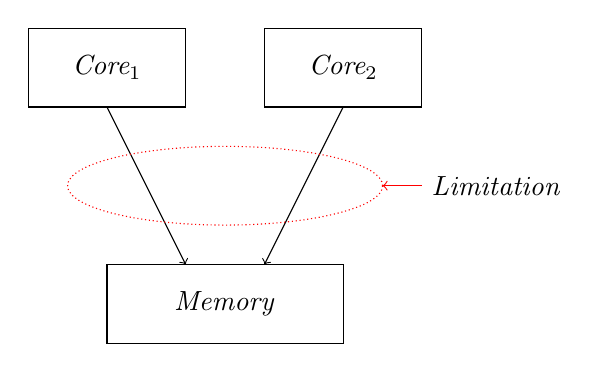
\begin{tikzpicture}
			\draw (1, 0) rectangle (4, 1) node[pos = 0.5]{\textit{Memory}};
			\draw (0, 3) rectangle (2, 4) node[pos = 0.5]{\textit{Core$_1$}};
			\draw (3, 3) rectangle (5, 4) node[pos = 0.5]{\textit{Core$_2$}};

			\draw[->] (1, 3) -- (2, 1);
			\draw[->] (4, 3) -- (3, 1);

			\draw[red, densely dotted] (2.5, 2) ellipse (2 and 0.5);
			\draw[red, <-] (4.5, 2) -- (5, 2) node[black, right]{\textit{Limitation}};
		\end{tikzpicture}
		\caption{Bottleneck of parallelized code.}
		\label{fig:parallelismbottleneck}
	\end{figure}	
}
